%\section{Einleitung}
\subsection{Schichtenarchitektur}
\begin{frame}
  \frametitle{Schichtenarchitektur}
  \framesubtitle{Definition}
  \begin{itemize}
    \item Hierarchische Struktur 
    \item Definiert Abstraktionsebenen mit allgemeinen Schnittstellen
    \item Jede Schicht repräsentiert ein Set von Funktionen
    \item Jede Schicht hat eine oder mehrere Interpretationen
    \item Jede Interpretation implementiert Protokolle 
  \end{itemize}
\end{frame}
\begin{frame}
  \frametitle{Schichtenarchitektur}
  \framesubtitle{Bedeutung}
  \begin{itemize}
    \item Komplexe Systeme in kleinere, einfachere Teile zerlegen
    \item Trennung von Verantwortlichkeiten 
    \item Schichten können unabhängig entwickelt, getestet und gewartet werden
    \item Jede Schicht kann als Komponente verstanden werden
    \item Interoperabilität und Kompatibilität steigt
    \item Wiederverwendbarkeit steigt 
    \item Chance und Risiko für Sicherheit
    \item Historisch wichtig und immer noch hohen Einfluss
  \end{itemize}
\end{frame}
\begin{frame}
  \frametitle{Schichtenarchitektur}
  \framesubtitle{Beispiele}
  \begin{itemize}
    \item ISO OSI Referenzmodell
    \item DECnet
    \item Cloud Architekturen
    \item Micro Service Architekturen
  \end{itemize}
\end{frame}

\begin{frame}
  \frametitle{Layer}
  \framesubtitle{Definition}
  \begin{itemize}
    \item Logische Gruppierung von Funktionen
    \item Schichten werden in der Regel vertikal angeordnet
    \item Jede Schicht erfüllt eine spezifische Funktion
  \end{itemize}
\end{frame}

\begin{frame}
  \frametitle{Layer}
  \framesubtitle{Beispiel}
  \begin{itemize}
    \item Presentation Layer
    \item Business Logic Layer
    \item Data Access Layer
  \end{itemize}
\end{frame}


\begin{frame}
  \frametitle{Layer}
  \framesubtitle{Als Komponenten}
  \begin{figure}[!h]
    \centering
    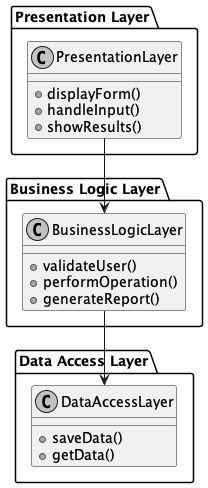
\includegraphics[width=0.20\textwidth]{fig/uml/simple-layers.png}
    \caption{Einfaches Schichtenmodell}
    \label{fig:simple-layer}
  \end{figure}
\end{frame}

\begin{frame}
  \frametitle{Tier}
  \framesubtitle{Definition}
  \begin{itemize}
    \item Physische oder logische Aufteilung
    \item Jedes Tier hat normalerweise eine spezifische Funktion 
    \item Normalerweise durch eine Netzwerkverbindung miteinander verbunden
  \end{itemize}
\end{frame}

\begin{frame}
  \frametitle{Tier}
  \framesubtitle{Beispiel}
  \begin{itemize}
    \item Präsentations-Tier
    \item Anwendungs-Tier 
    \item Datenbank-Tier
  \end{itemize}
\end{frame}

\begin{frame}
  \frametitle{Tier}
  \framesubtitle{Als Komponenten}

  \begin{figure}[!h]
    \centering
    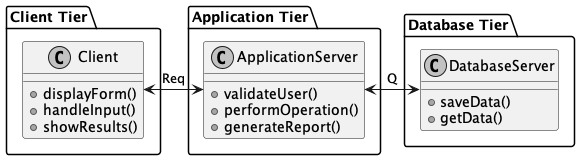
\includegraphics[width=0.95\textwidth]{fig/uml/simple-tiers.png}
    \caption{Einfaches Tier Modell}
    \label{fig:simple-tier}
  \end{figure}
\end{frame}